\documentclass[conference]{IEEEtran}
\IEEEoverridecommandlockouts
% The preceding line is only needed to identify funding in the first footnote. If that is unneeded, please comment it out.
\usepackage{cite}
\usepackage{amsmath,amssymb,amsfonts}
\usepackage{algorithm}
\usepackage{algpseudocode}
\usepackage{graphicx}
\usepackage{textcomp}
\usepackage{xcolor}
\usepackage{subcaption}
\usepackage{hyperref}

\def\BibTeX{{\rm B\kern-.05em{\sc i\kern-.025em b}\kern-.08em
    T\kern-.1667em\lower.7ex\hbox{E}\kern-.125emX}}
\begin{document}

\title{ECE276B PR3 Report}

\author{
\IEEEauthorblockN{1\textsuperscript{st} Weixiao Zhan}
\IEEEauthorblockA{
    weixiao-zhan[at]ucsd[dot]edu}
}

\maketitle

\section{Introduction}
This project aims to develop a safe trajectory tracking policy 
for a ground differential-drive robot.
The trajectory tracking problem is formulated as a 
discounted infinite-horizon stochastic optimal control problem.
The control policy must track a periodic reference trajectory 
while managing motion model noise and avoiding obstacles. 

This project explores two primary approaches: 
receding-horizon certainty equivalent control (CEC) and 
generalized policy iteration (GPI), specifically the Q-value iteration. 
The performance of both methods is evaluated based on 
tracking accuracy, computational complexity, and collision avoidance capabilities.


\section{Problem Formulation}
\subsection{Environment}
The environment, which the robot operates in, is 
a \(xy\)-plane bounded within \([-3, 3] \times [-3, 3]\).
There are two circular obstacles:
Obstacle \( C_1 \) centered at \((-2, -2)\) with a radius of 0.5.
Obstacle \( C_2 \) centered at \((1, 2)\) with a radius of 0.5.
Denote the free space:
\[ \mathcal{F} = [-3, 3]^2 \setminus (C_1 \cup C_2) \]

The reference trajectory is a sequence of positions and orientations:
\[ r_t \in [-3,3] \times [-3,3] \times [-\pi, \pi), t < \mathcal{T}\]
with period $\mathcal{T}$ and may overlap with obstacles.

\subsection{Motion Model}
The motion model of the differential-drive robot is defined as follows. 
The robot's state at time \( t \), denoted by 
\( {x}_t = [\begin{matrix}{p}_t & \theta_t\end{matrix}]^T \), 
consists of position \( {p}_t \in \mathcal{F} \) and orientation \( \theta_t \in \mathbb{R} \). 
The control input \( {u}_t = (v_t, \omega_t) \) 
consists of the linear velocity \( v_t \in [0,1] \) and 
angular velocity \( \omega_t \in [-1,1] \). 
The motion model, with time interval \( \Delta > 0 \), is:

\[
{x}_{t+1} = {f}({x}_t, {u}_t, {w}_t) = {x}_t + {G}({x}_t) {u}_t + {w}_t
\]
where
\[
{G}({x}_t) = \begin{bmatrix}
\Delta \cos(\theta_t) & 0 \\
\Delta \sin(\theta_t) & 0 \\
0 & \Delta 
\end{bmatrix}
\]
and motion noise \( {w}_t \sim \mathcal{N}(0, \Sigma) \).

\subsection{Receding-horizon CEC}
CEC is a suboptimal open-loop-feedback control scheme.
At each stage, it applies the control that would be optimal,
if the noise variable $w_t$ were realized at their expected values. 
The main advantage of CEC is that it reduces 
a stochastic optimal control problem to a deterministic optimal control problem, 
which can be solved more efficiently. 

In addition,
receding-horizon CEC approximates infinite-horizon problem 
by repeatedly solving a discounted finite-horizon
deterministic optimal control problem, with look ahead steps $T$, at each time step.

Formally, when given state $x_\tau$, 
CEC solves following optimization problem to find control sequence $u_{\tau:\tau+T-1}$, 
applies the first control $u_\tau$. 
At next stage, repeat this process with $x_{\tau+1}$.
\[
\begin{gathered}
\min_{{u}_\tau, \ldots, {u}_{\tau+T-1}} 
q({e}_{\tau+T}) + 
\sum_{t=\tau}^{\tau+T-1} \gamma^{t-\tau} 
\left( 
    \begin{gathered}
        \tilde{p}_t^\top Q \tilde{p}_t  \\ 
        +\\
        q(1 - \cos(\tilde{\theta}_t))^2 \\
        +\\
        {u}_t^\top R {u}_t 
    \end{gathered} 
\right) \\
s.t. \left\{
\begin{aligned}
{e}_{t} 
    &= x_{t} - r_{t} \\
    &= \left[\begin{matrix}\tilde{p}_t&\tilde{\theta}_t\end{matrix}\right]^T \\
x_{t} 
    &= f({x}_{t-1}, {u}_{t-1}, 0) \\
    &= \left[ \begin{matrix}p_{t} & \theta_{t} \end{matrix}  \right]^T \\
{p}_t
    &\in \mathcal{F} \\
{u}_t
    &\in \mathcal{U} \\
\end{aligned}
\middle|
\begin{aligned}
    x_\tau\\
    T &\in \mathbb{N}^+\\
    Q &\in \mathbb{R}^{[2\times 2]} \\
    q &\in \mathbb{R} \\
    R &\in \mathbb{R}^{[2\times 2]}
\end{aligned}
\right.
\end{gathered}
\]
in which, $q$ is the terminal cost, 
$Q,q,R$ are stage cost hyper-parameters.

\subsection{Non-linear Programming (NLP)}
An NLP program written in following standard form can be solved by an NLP solver.
\[
\begin{aligned}
&\min_{{U}} & & c({U}, {E}) \\
&\text{subject to} & & {U}_{\text{lb}} \leq {U} \leq {U}_{\text{ub}} \\
& & & {h}_{\text{lb}} \leq {h}({U}, {E}) \leq {h}_{\text{ub}}
\end{aligned}
\]
where \( {U} = [{u}_\tau^\top, \ldots, {u}_{\tau+T-1}^\top]^\top \) and \( {E} = [{e}_\tau^\top, \ldots, {e}_{\tau+T}^\top]^\top \).

\subsection{GPI}
GPI is a powerful technique to approach 
infinite horizon planing problem.
The standard GPI repeats following two steps until converged:
\subsubsection{policy evaluation} try to find value function $V^{\pi}$ of a given policy $\pi$.
\subsubsection{policy improvements} greedy improve the policy.

To use GPI in contiguous state space, 
discretization or parametrization of value function are necessary.

\subsection{Q-value iteration}
Q-value iteration is an equivalent variation of general policy iteration.
Its routines is shown in Algorithm \ref{algo:gpi}.
\begin{algorithm}
    \caption{Q-value iteration}
    \label{algo:gpi}
    \begin{algorithmic}[1] % The number [1] enables line numbering
    \While{$\delta Q > \epsilon$}
        \Comment Q-value iteration
        \State for $\forall x \in \mathcal{X}, u \in \mathcal{U}$
        \State $Q(x,u) = l(x,u) + \gamma \mathbb{E}_{x'\sim p_f}\left[\min_{\forall u' \in \mathcal{U}} Q(x', u')\right]$
        % Your loop code here
    \EndWhile
    \State $\pi(x) \leftarrow \arg\min_u Q(x, u), \forall x$
    \Comment extract policy
    \end{algorithmic}
\end{algorithm}


\section{Technical Approach}

\subsection{Receding-horizon CEC: NLP Formulation}
In this project, the receding-horizon CEC problem is converted into standard NLP form and solved using Casadi library.

\subsubsection{optimization variable}
\[
\begin{aligned}
U&=\left[ \begin{matrix}u_{\tau }&...&u_{\tau +T-1}\end{matrix}  \right] &\in R^{[2\times T]}\\ 
U_{lb}&=\left[ \begin{matrix}0&\cdots &0\\ -1&\cdots &-1\end{matrix}  \right] \\ 
U_{ub}&=\left[ \begin{matrix}1&\cdots &1\\ 1&\cdots &1\end{matrix}  \right] 
\end{aligned} 
\]

\subsubsection{objective}
\[
\begin{gathered}
\begin{aligned}
C(U, x_\tau)
    &=\sum^{\tau +T-1}_{t=\tau } \gamma^{t-\tau } \cdot \left(loss_{e}\left( x_{t}-r_{t} \right) +loss_{u}\left( u_{t} \right)  \right) \\
\end{aligned}
\\ 
\text{in which} \left\{\begin{aligned}
loss_{e}(e_{t})
    &=\underbrace{\tilde{p}^{T}_{t}Q\tilde{p}_{t}}_{A} 
    +\underbrace{q\left( 1-\cos \left( \tilde{\theta}_{t}  \right)  \right)^{2} }_{B} \\ 
loss_{u}(u_{t})
    &=\underbrace{u^{T}_{t}Ru_{t}}_{C} 
    +\underbrace{\left( u_{t}-u_{t-1} \right)^{T} r\left( u_{t}-u_{t-1} \right) }_{D} \\
x_{t}&=f(x_{t-1},u_{t})\\ 
e_{t}&=\left[ \begin{gathered}\tilde{p}_{t}\\ \tilde{\theta}_{t} \end{gathered}  \right]
\end{aligned} \right.
\end{gathered}
\]

The above Formulation hardcoded the motion model $f$, reference trajectory $r_t$,
and error state $e_t$'s calculation into the objective function. 

Term $A$ and $B$ regulates the position and orientation error 
between states and reference trajectory.
Term $C$ regulates large controls.

Term $D$ is an added smoothing term.
It regulates the controls' change rate to avoid sharp turns.
Its impact is further discussed in Results section.

\subsubsection{constrains}
\[
\begin{gathered}
\begin{aligned}
h(U, x_\tau)&=\left[ \begin{matrix}p_{\tau +1}&\cdots &p_{\tau +T-1}\\ \| p_{t}-c_{1}\|_{2} &\cdots &\| p_{\tau +T-1}-c_{1}\|_{2} \\ \| p_{t}-c_{2}\|_{2} &\cdots &\| p_{\tau +T-1}-c_{2}\|_2 \end{matrix}  \right] \\ 
h_{lb}&=\left[ \begin{matrix}\left[ \begin{gathered}-3\\ -3 \end{gathered}  \right] &\cdots &\left[ \begin{gathered}-3\\ -3 \end{gathered}  \right] \\ c_{1}.radius&\cdots &c_{1}.radius\\ c_{2}.radius&\cdots &c_{2}.radius\end{matrix}  \right] \\ 
h_{ub}&=\left[ \begin{matrix}\left[ \begin{gathered} 3\\  3 \end{gathered}  \right] &\cdots &\left[ \begin{gathered} 3\\  3 \end{gathered}  \right] \\ \infty&\cdots &\infty\\ \infty&\cdots &\infty\end{matrix}  \right] 
\end{aligned} \\
\end{gathered} 
\]
in which, 
\( x_{t} = \left[ \begin{gathered}p_{t}\\ \theta_{t} \end{gathered}  \right]  
=f(x_{t-1},u_{t-1}) \)

Similar to objective function, the motion model $f$ is hardcoded into the constrain function.
The constrains enforce states $x_{\tau+1:\tau+T-1}$ to be within the free space $\mathcal{F}$.

\subsubsection{formation considerations}
Converting CEC into the above NLP without explicitly introducing 
optimization variable on state $x_t$ or error states $e_t$ has several benefits.
\begin{itemize}
    \item avoids motion model constrains in following form: 
    \[-\epsilon < x_{t+1} - f(x_t, u_t) <\epsilon\]
    \item avoids implementing error state motion model.
    \item avoids boundary and collision check on error states $e_t$.
    \end{itemize}

The formulation does not normalize the orientation $\theta_t$ into the reference trajectory's orientation space $[-\pi, \pi)$,
as the objective function has taken periodic $\cos$ over $\tilde{\theta}$.

The formulation also skipped stage cost.
A conventional stage cost $q(x_{\tau+T}) = \gamma^T (loss_e(e_{\tau+T}) + loss_u(u_{\tau+T}))$
would have the same effect of increasing look ahead step by 1, thus skipped.

\subsubsection{hyper-parameter tuning}
In practice, following hyper-parameters produced best results:
\[
\begin{array}{ll}
    T=5
    &\gamma = 0.9\\ 
    Q=\left[ \begin{matrix}2&0\\ 0&2\end{matrix}  \right] 
    &q=2\\ 
    R=\left[ \begin{matrix}0.05&0\\ 0&0.05\end{matrix}  \right] 
    &r=\left[ \begin{matrix}0.05&0\\ 0&0.05\end{matrix}  \right] 
\end{array} 
\]
Different hyper-parameters and their effect are further discussed in Results section.

\subsection{GPI: GPU Batch Q-value iteration}
The computation of Q-value iteration is highly parallelizable, 
making GPUs the ideal hardware to leverage. 
In this project, 
a GPU-accelerated batch Q-value iteration is implemented with PyTorch.

\subsubsection{state space and control space discretization}
The orientation is first normalized into $[-\pi,\pi)$.
The state space $\mathcal{X} = [-3,3]^2\times[-\pi,\pi)$ is
discretized into $(nx, ny, nth)$ equally-spaced points in each dimension.
The control space $\mathcal{U} = [0,1]\times[-1,1]$ is discretized into $(nv,nw)$
equally-spaced controls values.
Since the trajectory has period $\mathcal{T}$, 
the time horizon is discretized in $nt=\mathcal{T}$ steps.

\subsubsection{f:transition matrix and probability}
The continuous and stochastic motion model
\[p_f(\cdot | x, u, w) \]
is discretized and approximated using the following method:

\begin{itemize}
    \item For all discrete state \( x \) and control \( u \),
    a neighborhood with $K$ discrete states, denote as \( \{x'_{k} |k < K\}\), 
    around the next state's expectation, \(x' = f(x, u, 0) \)
    is considered possible next states.
    \item The neighborhood selection make sure the positions $p'_k$ are clamped between $[-3,3]^2$
    and the orientations $\theta'_k$ are wrapped around. 
    \item  The likelihood of transitioning into \( x'_k \)
    is evaluated using Gaussian distribution
    \footnote{The motion model $f$ is not linear, but we will assume it is, and approximated 
    the result distribution with Gaussian distribution.}
    \( N(x', \Sigma) \).
    \item The transition probability distribution is normalized 
    \footnote{The torch normalization function will correctly return all zero if the input is all zero}
    within the neighborhood, so that \(\sum_k Prob(x'_{k}) = 1\).
\end{itemize}

The discretization of $f$ can be efficiently computed with PyTorch batch and broad cast operations.
The results are saved in two tensors:
transition tensor $P$ with shape $(K, nx, ny, nth, nv, nw, 3)$ 
stores the \textbf{indices} of neighborhood points $x'_k$;
transition probabilities tensor $P_p$ with shape $(K, nx, ny, ,nth, nv, nw)$ 
stores their probabilities.

The transition tensors are discretization of $f$, thus is \textbf{time invariant}.

\subsubsection{stage cost}
$$
\begin{aligned}
l(x_t, u_t) &= 
    \tilde{p}^{T}_{t}Q\tilde{p}_{t} 
    + q\left( 1-\cos \left( \tilde{\theta}_{t}  \right)  \right)^{2} 
    + u^{T}_{t}Ru_{t} \\
s.t. \ \left[ \begin{gathered}\tilde{p}_{t}\\ \tilde{\theta}_{t} \end{gathered}  \right] 
    &= x_{t}-r_{t}
\end{aligned}
$$

The stage cost can be discretized and saved to tensor $L$ with shape $(nt, nx, ny, nth, nv, nw)$.
For those states that are on the boundary and causing collision, 
their stage costs are set to $\infty$.
The stage cost dependents on the reference trajectory and is \textbf{time variant}.

\subsubsection{Q-value iteration and policy extraction}
implements Algorithm \ref{algo:gpi} using batch operations.
It first computes current V-values $V = \min_{\text{dim}=[-2,-1]} Q$.
The expectation $E_{x' \sim p_f}$ is approximated by the weighted sum of 
neighborhoods' V-values at next time step $t' = (t+1)\mod nt$.
Q values are stored in tensor $Q$, with shape $(nt, nx, ny, nth, nv, nw)$.

Q value iteration is executed until $\|Q_k - Q_{k-1}\| < \delta$.
Then the policy $\pi$ is extracted: $\pi = \arg\min_{\text{dim}=[-2,-1]} Q$.

\subsubsection{implementation considerations}
Similar to CEC approach, 
standard states and motion model $f$ is discretized instead of error states.
The primary considerations is memory consumption.
The standard motion model need to discrete $6*6*2\pi*1*2$ hyper-volume 
but the error motion model need to discrete $12*12*2\pi*1*2$ hyper-volume which is 4 times greater.

However, the error state allows adaptive discretization: 
discrete finer near the origin and coarse on the peripheral, 
which is left for future work.

\subsubsection{hyper-parameter tuning}
In practice, GPI used the same $Q,q,R$ as CEC. 
And following discretization perform the best:
\[
\begin{array}{lll}
nt=100&&\\ 
nx=31&ny=31&nth=11\\ 
nv=6&nw=11&\\
K=1&\delta = 10\end{array} 
\]

Because the discretization is relatively sparse compare to the noise variance,
most of the probability weight is concentrated on one or two points in the neighborhood.
A 7-point spindle neighborhood ($K=7$) would have $7\times$ peak memory consumption
\footnote{A non-batch or subdivided batch Q iteration would have smaller peak memory consumption, 
but due to time limits and left for future work.}
compare to $K=1$ neighborhood in batch Q iteration,
which unfortunately exceeded my GPU GRAM capacity.
Thus the nearest point neighborhood ($K=1$) is used.

Those infinite stage costs are set to a large number of $10^{10}$, 
as infinity cause \texttt{nan} in computation.
With $\delta=10$, Q-value iteration takes around 50 iterations to converge.

\section{Results}
Best results of using P-controller CEC, and GPI are present in Figure \ref{fig:best}.
Both CEC and GPI are able to track the reference trajectory and avoid obstacles.
Full animated results can be found at \texttt{fig/*.gif}.

\begin{figure*}
    \centering
    \begin{subfigure}[b]{0.3\textwidth}
        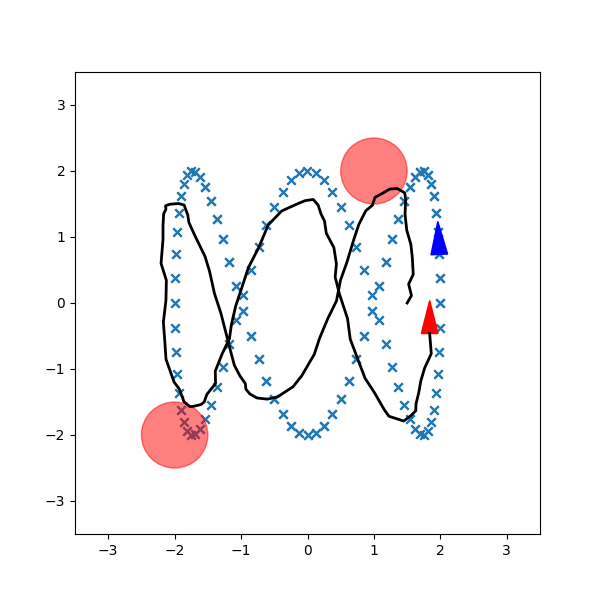
\includegraphics[width=\textwidth]{../fig/p_controller.png}
        \caption{p-controller}
        \label{fig:p-controller}
    \end{subfigure}
    \hfill
    \begin{subfigure}[b]{0.3\textwidth}
        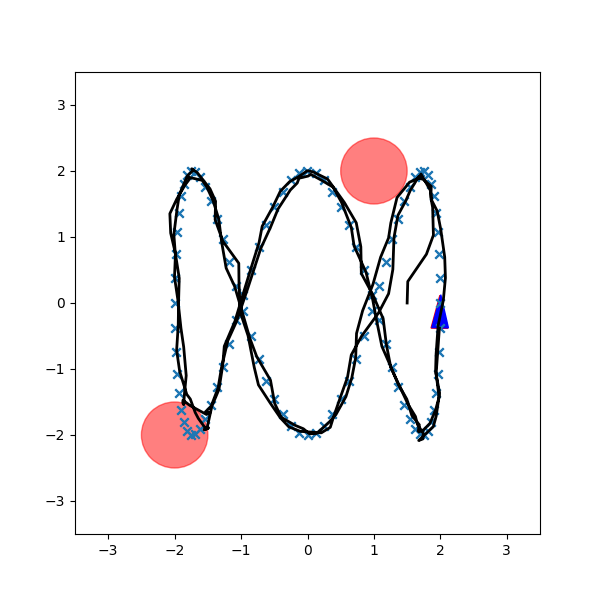
\includegraphics[width=\textwidth]{../fig/trajectory.cec.png}
        \caption{CEC}
        \label{fig:cec}
    \end{subfigure}
    \hfill
    \begin{subfigure}[b]{0.3\textwidth}
        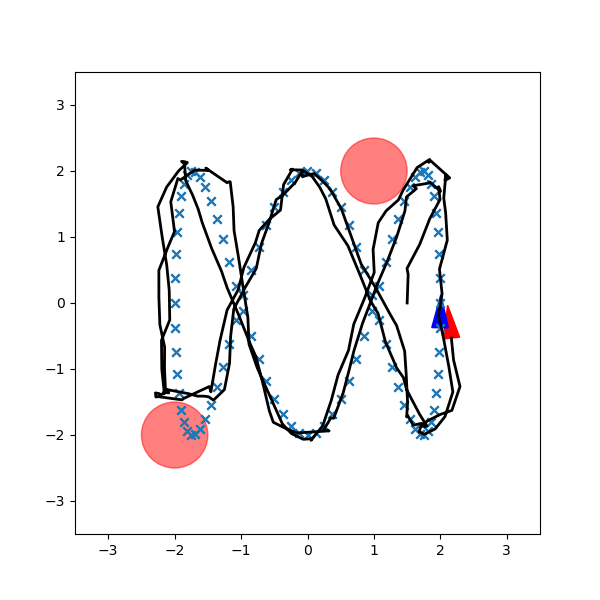
\includegraphics[width=\textwidth]{../fig/trajectory.gpi.png}
        \caption{GPI}
        \label{fig:gpi}
    \end{subfigure}
    \caption{Best results from CEC, GPI}
    \label{fig:best}
\end{figure*}

\subsection{CEC}
This section compares results produced by different hyper-parameters of CEC.

\subsubsection{look ahead steps}
Figure \ref{fig:Ts} shows the effect of changing $T$.
Compare to $T=5$ (Figure \ref{fig:T5}),
Too small $T=1$ (Figure \ref{fig:T1}) caused the policy can't avoid obstacles in advance.
Too large $T=20$ (Figure \ref{fig:T1}) caused the solver converged to a different optimal, 
it first bypassed the obstacles then chase the trajectory. 
This could due the choose of $\gamma = 0.9$, 
the solver didn't weight the near stages enough.

In addition, larger $T$ cause CEC slower to solve. 
$T=25$ is around the limit of finding next control in time on my machine.

\begin{figure*}[h]
    \centering
    \begin{subfigure}[b]{0.3\textwidth}
        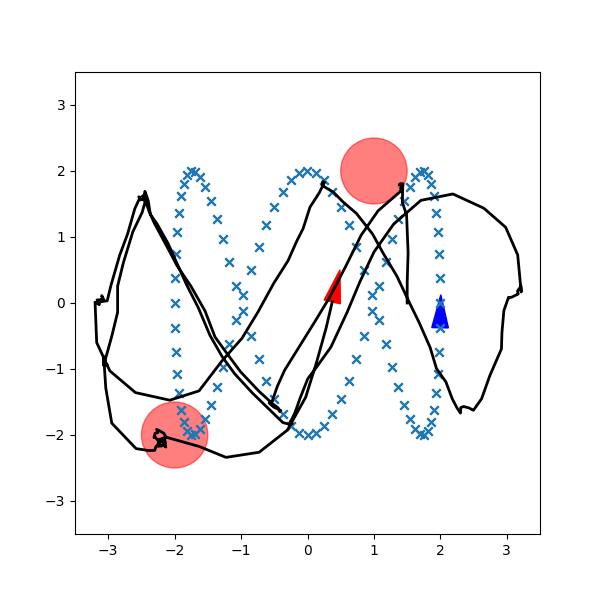
\includegraphics[width=\textwidth]{../fig/trajectory.cec.T_1.png}
        \caption{$T=1$}
        \label{fig:T1}
    \end{subfigure}
    \hfill
    \begin{subfigure}[b]{0.3\textwidth}
        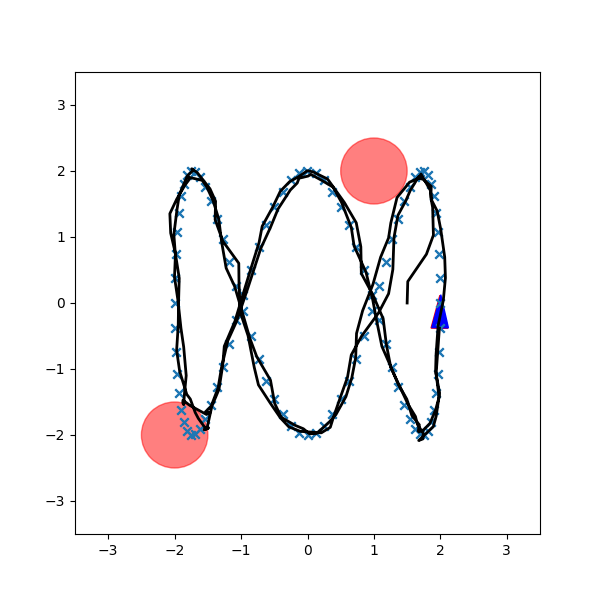
\includegraphics[width=\textwidth]{../fig/trajectory.cec.png}
        \caption{base line $T=5$}
        \label{fig:T5}
    \end{subfigure}
    \hfill
    \begin{subfigure}[b]{0.3\textwidth}
        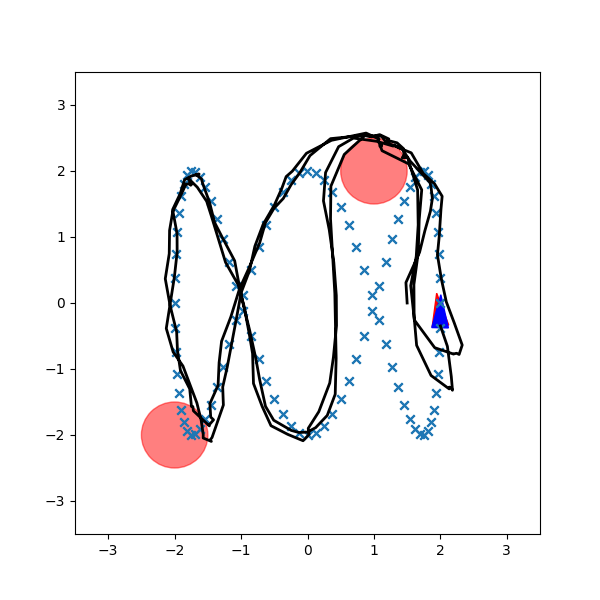
\includegraphics[width=\textwidth]{../fig/trajectory.cec.T_20_0.1.png}
        \caption{$T=20$}
        \label{fig:T20}
    \end{subfigure}
    \caption{look ahead steps}
    \label{fig:Ts}
\end{figure*}

\subsubsection{smoothing term}
In the CEC formation, a smoothing term $D$ is added.
Figure \ref{fig:r} shows the result without smoothing and with $r=1$ compare to $r=0.05$ at \ref{fig:r005}.
With the smoothing term, the turns are less sharp.
For a different less smooth reference trajectory, such smoothing term could become useful.

\begin{figure*}[h]
    \centering
    \begin{subfigure}[b]{0.3\textwidth}
        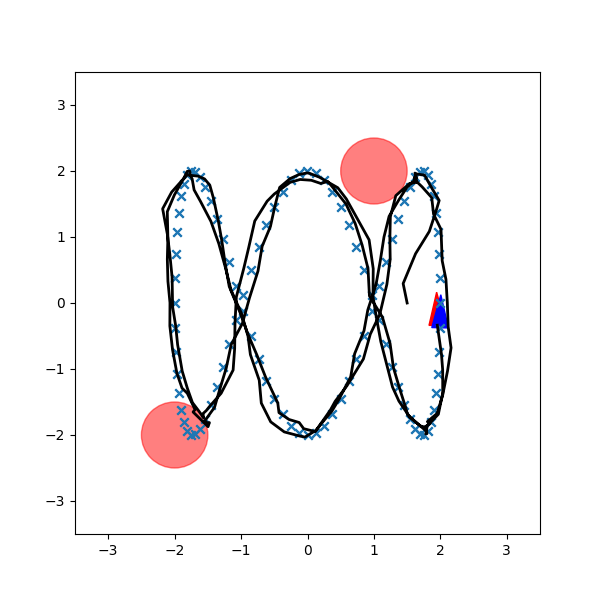
\includegraphics[width=\textwidth]{../fig/trajectory.cec.r_0.png}
        \caption{no smoothing $r=0$}
        \label{fig:r0}
    \end{subfigure}
    \hfill
    \begin{subfigure}[b]{0.3\textwidth}
        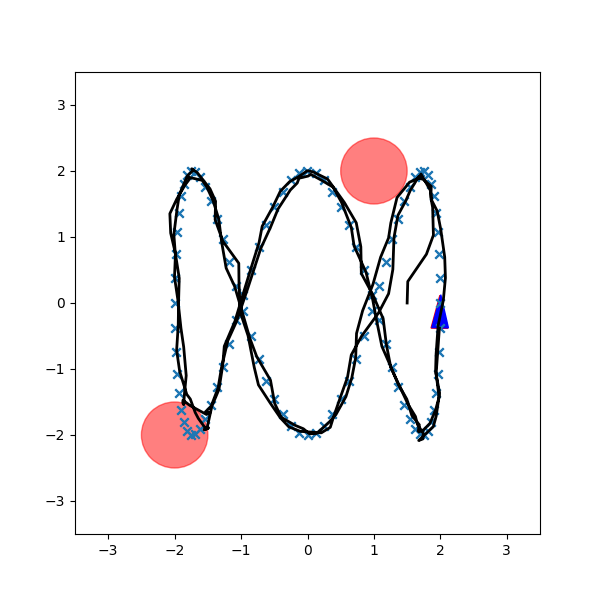
\includegraphics[width=\textwidth]{../fig/trajectory.cec.png}
        \caption{base line $r=0.05$}
        \label{fig:r005}
    \end{subfigure}
    \hfill
    \begin{subfigure}[b]{0.3\textwidth}
        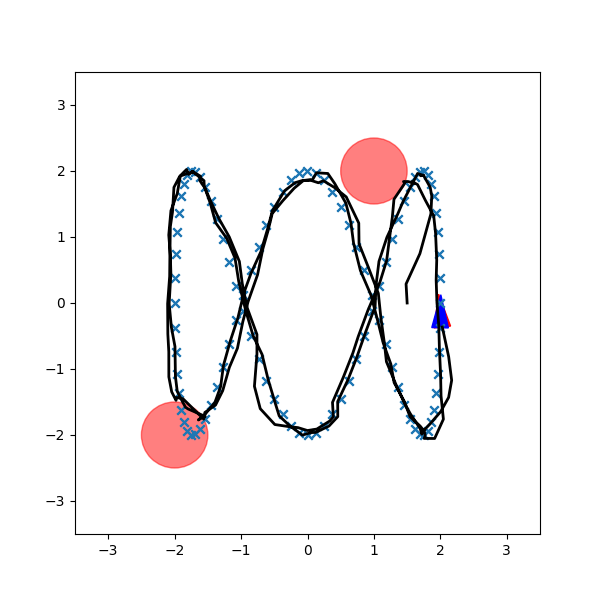
\includegraphics[width=\textwidth]{../fig/trajectory.cec.r_1.png}
        \caption{more smoothing $r=1$}
        \label{fig:r1}
    \end{subfigure}
    \caption{smoothing term}
    \label{fig:r}
\end{figure*}

\subsubsection{less important: $\gamma, q$}
Figure \ref{fig:p} shows two less important parameters.
Non-discounted result ($\gamma = 1$ at Figure \ref{fig:gamma1}) is really close to the baseline result with $\gamma = 0.9$.
Figure \ref{fig:q0} shows the orientation term B is also less import in this project,
because the reference orientation is always the tangent direction of reference trajectory.
For a different motion model with degree of freedom in orientation, term B would be more significant.

\begin{figure*}[h]
    \centering
    \begin{subfigure}[b]{0.3\textwidth}
        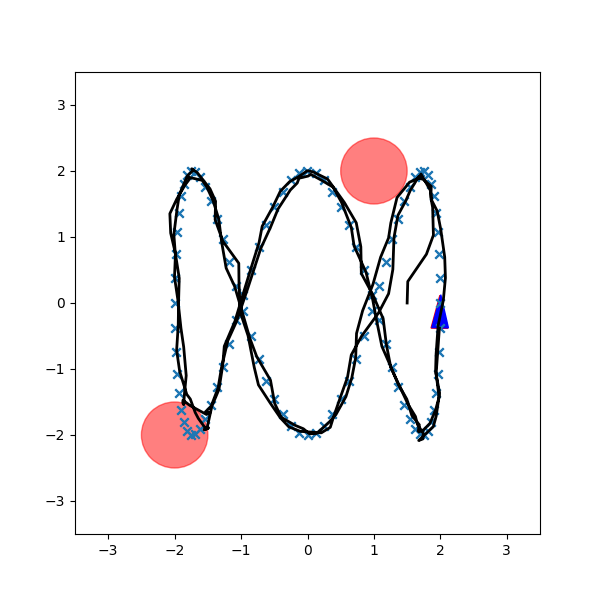
\includegraphics[width=\textwidth]{../fig/trajectory.cec.png}
        \caption{base line, $q=2, \gamma=0.9$}
        \label{fig:base}
        \end{subfigure}
    \hfill
    \begin{subfigure}[b]{0.3\textwidth}
        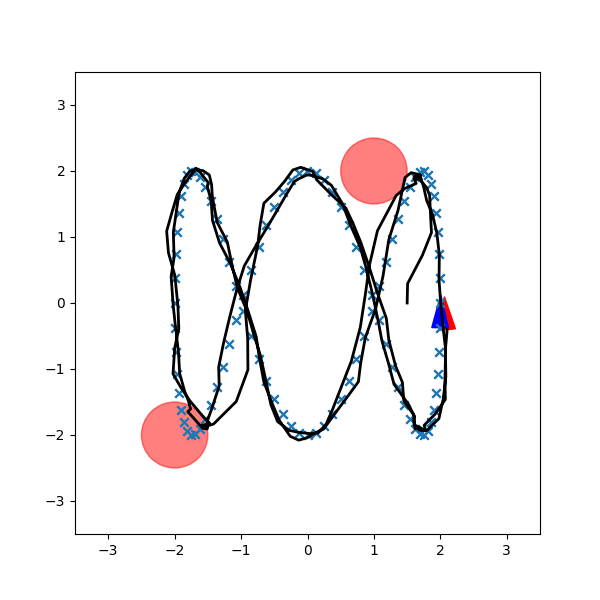
\includegraphics[width=\textwidth]{../fig/trajectory.cec.q_0.png}
        \caption{$q=0$}
        \label{fig:q0}
    \end{subfigure}
    \hfill
    \begin{subfigure}[b]{0.3\textwidth}
        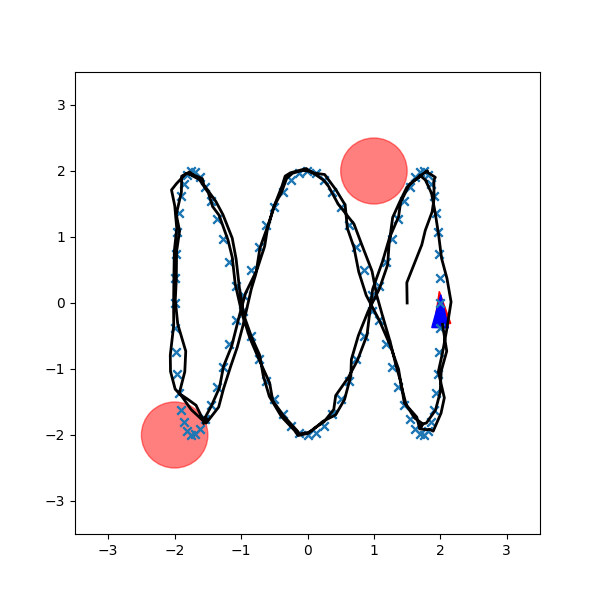
\includegraphics[width=\textwidth]{../fig/trajectory.cec.gamma_1.png}
        \caption{$\gamma=1$}
        \label{fig:gamma1}
    \end{subfigure}
    \caption{less important parameters}
    \label{fig:p}
\end{figure*}

\subsection{GPI}
Figure \ref{fig:gpi} shows the result of optimal policy extracted from Q-value iteration.
Compare to CEC results, it is clear that due to discretization granularity 
the GPI's control is less refined. However, the advantage of GPI is it online runtime.
Only one table lookup can decide the current control, which can be significant in 
latency sensitive and small time interval applications.
\end{document}
